\chapter{Introduction}
Since the seminal report by \citet{Reid1910}, it has been recognized
that earthquakes are caused by the sudden release of elastic strain
energy that has gradually accumulated over time along faults. This is
known as elastic rebound theory. \citet{Reid1910} introduced elastic
rebound theory to explain ground deformation leading up to and as a
result of the 1906 San Francisco earthquake. In the report,
triangulation surveys showed that the ground on either side of the San
Andreas fault and at far distances from the fault was steadily
undergoing a shearing motion at a rate of about 6 cm/year. During the
1906 earthquake, the San Andreas fault slipped by about 6 meters,
presumably releasing the elastic strain energy in the crust that has
accumulated over the past hundred years or so. Modern geodetic
techniques have updated the rate of deformation across the San Andreas
fault to about 3 cm/year \citep{Savage1973}, but elastic rebound
theory has remained generally accepted since its inception over a
century ago.

Elastic rebound theory forms the foundation of seismic hazard models
such as the third Unified California Earthquake Rupture Forecast
(UCERF3) \citep{Field2014}. Geodetic observations can tell us the rate
that strain is accumulating between tectonic plates. Based on elastic
rebound theory, this built up strain will inevitably be relaxed through
fault slip. It is then possible to use geodetic data to estimate the
long term fault slip rates that are needed to accommodate tectonically
accumulated strain \citep[e.g.,][]{Savage1973,Meade2005}. UCERF3 uses
geodetically and geologically derived slip rates for the San Andreas
Fault system in conjunction with various other assumptions to estimate
the likelihood that a major earthquake would occur over some window of
time in California. UCERF3 has clear societal implications; it is used
by engineers for designing buildings, and it is used by the California
Earthquake Authority for determining earthquake insurance rates.

In constraining UCERF3, it is assumed that strain is building up on
the San Andreas fault system at a constant rate over time. However,
time-dependent, or transient, deformation around fault zones is a
frequently observed phenomena that casts doubt into this assumption
\citep{Thatcher1983}. By better understanding transient deformation
and the mechanisms causing it, we can then conceivably improve upon
existing seismic hazard models. Some of the earlier records of
transient deformation came from repeated leveling or triangulation
surveys made after large earthquakes \citep[e.g.,][]{Tsuboi1932,
Smith1968}. These studies revealed elevated rates of ground
deformation following the earthquakes, which then decayed over a
timescale of months to years. This type of transient deformation is
referred to as postseismic deformation.

Over the past few decades, Global Navigation Satellite Systems
(GNSS)\footnote{The terms ``GNSS" and ``GPS" (Global Positioning
System) will be used synonymously in this dissertation, although GPS
is specifically operated by the United States and GNSS is a more
generic term.} have become a valuable geodetic tool for observing
transient deformation. Throughout most of the 20th century, geodetic
techniques, such as triangulation and leveling surveys, required
someone to be physically present at the geodetic monuments in order to
make an observation. Consequently, the time interval between
consecutive observations tended to be on the order of months to years.
Using a GNSS receiver that has been specialized for geodetic purposes,
observations of ground displacements can be made automatically with
sampling frequencies greater than 1Hz. The accuracy of GNSS
measurements is also unprecedented, where the uncertainties for daily
displacement observations tend to be on the order of a couple
millimeters. The advent of GNSS geodesy has led to numerous
geophysical discoveries. For example, \citet{Dragert2001} discovered
slow slip events on the Cascadia subduction zone using daily GNSS
observations in the Pacific Northwest. These slow slip events produce
several millimeters of ground deformation over the course of a couple
weeks. As another example, \citet{Freed2007} discovered far reaching
postseismic deformation following the 1999 Hector Mine earthquake
using GNSS data. They were able to resolve several millimeters of
ground deformation over 200 km from the earthquake's epicenter, which
occurred during the seven years following the earthquake.

The recently installed Plate Boundary Observatory (PBO) has
substantially improved our ability to resolve transient deformation in
the western United States, which is where I am primarily focused in
this dissertation. The PBO consists of about 1100 continuously
operating GNSS stations and about 80 borehole strainmeters (BSMs) that
have been placed along the boundary between the Pacific and North
American plate. Construction of the PBO began in 2003 and lasted until
2008. Today, the PBO instruments are being actively maintained by
UNAVCO. There is a wealth of geodetic data collected by the PBO, and
geophysicists have been using the data to refine our understanding of
tectonic and volcanic processes.

In this dissertation I study transient deformation associated with
tectonic processes, such as postseismic deformation and slow slip
events. The immediate objective of this dissertation is to detect
transient deformation and better understand the mechanisms causing it.
The broader motivation for my research is to improve our understanding
of earthquakes and seismic hazard. 


\section{Types of Transient Tectonic Deformation}
My focus is on transient ground deformation associated with tectonic
processes. Specifically, I will consider postseismic deformation,
interseismic deformation, and slow slip events. Transient deformation
resulting from volcanic, seasonal, or anthropogenic processes will
either be ignored or considered noise. The following sections further
discuss the processes considered in this dissertation.

\subsection{Postseismic deformation}
Postseismic deformation is the anomalously rapid ground deformation
observed after large earthquakes (M${\gtrsim}$6). Geodetic
observations made after the 1966 Parkfield earthquake provided one of
the first views of the time-dependence of postseismic deformation
\citep{Smith1968}. The Parkfield segment of the San Andreas fault is
the transition between the creeping segment in central California and
the locked segment in southern California, which last ruptured in the
1857 Fort Tejon earthquake. The Parkfield segment has produced seven
M6 earthquakes since 1857, and has consequently received much
attention from geophysicists. In the months after the 1966 earthquake,
\citet{Smith1968} observed 20 cm of ground displacements across the
San Andreas fault near the epicenter. The postseismic deformation was
most rapid (about 1 cm/day) immediately after the earthquake and
decayed logarithmically over time. The observed deformation was
localized to within tens of meters of the San Andreas fault trace,
which allowed \citet{Smith1968} to unambiguously conclude that the
postseismic deformation was primarily the result of aseismic fault
slip, referred to as afterslip (Figure \ref{intro:fig:1}).
Furthermore, it was determined that most of the fault slip during the
earthquake was at depth and the ensuing afterslip filled in the slip
deficit at shallower depths. Afterslip has also been used to describe
postseismic deformation following the subsequent Parkfield earthquake
in 2004 \citep{Freed2007}.

Postseismic deformation following larger California earthquakes has
also been explained with afterslip, such as the M7.3 Landers
earthquake \citep{Shen1994, Savage1997}, the M7.1 Hector Mine
earthquake \citep{Jacobs2002, Owen2002}, and the M7.2 El Mayor-Cucapah
earthquake \citep{Gonzalez-ortega2014}. The stress changes from these
earthquakes were potentially large enough to cause the asthenosphere
to viscously deform. This viscous relaxation of coseismic stresses
would then manifest as broad-scale postseismic deformation
\citep{Nur1974} (Figure \ref{intro:fig:1}). Postseismic deformation
resulting from viscous relaxation can be practically indistinguishable
from postseismic deformation resulting from afterslip that is occurring
below seismogenic depths \citep{Savage1990}. Indeed, researchers have
also been able to describe postseismic deformation following the
Landers, Hector Mine, and El Mayor-Cucapah earthquakes with viscous
relaxation in the upper mantle \citep{Pollitz2000, Pollitz2001,
Freed2004, Freed2007a, Spinler2015} or a combination of afterslip and
viscous relaxation \citep{Pollitz2012, Pollitz2015, Rollins2015}. It
is important to discern which mechanisms is driving postseismic
deformation because that information can shed light onto how stress is
building up on faults. Several researchers have suggested using the
polarity of vertical postseismic deformation as a discriminant for the
deformation mechanism \citep[e.g.,][]{Pollitz2003, Hetland2014,
Rollins2015}.

\begin{figure} 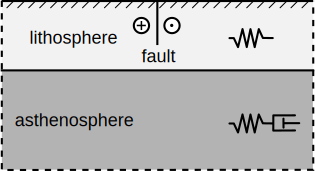
\includegraphics{schematic} 
\caption[Schematics of postseismic deformation mechanisms] 
{Schematics of postseismic deformation mechanisms. The left schematic
illustrates the viscous relaxation model, where an earthquake produces
fault slip in an elastic lithosphere that overlies a viscoelastic
asthenosphere. Stresses from the earthquake cause the asthenosphere to
flow which will then cause postseismic surface deformation. The right
schematic illustrates the afterslip model, where aseismic fault slip
(gray) occurs around the region that slipped during the earthquake
(black) to relieve coseismic stresses.}
\label{intro:fig:1}
\end{figure}

\subsection{Interseismic deformation} 
For the aforementioned California earthquakes, transient postseismic
deformation persisted over timescales of months to years. Postseismic
deformation subsides once the coseismic stresses have been dissipated
through viscous relaxation or afterslip. After that time, ground
deformation returns to a relatively steady rate. This relatively
steady deformation is referred to as interseismic deformation. I use
the term ``relatively steady" because interseismic deformation can
still exhibits transients. For example, \citet{Thatcher1983} observed
a decay in strain rates across the San Andreas fault that occurred
over the decades following the The 1906 San Francisco and 1857 Fort
Tejon earthquakes. \citet{Savage1978} introduced a model to describe
time-dependent interseismic deformation. In this model an elastic
lithosphere overlies a viscoelastic asthenosphere. The model is driven
by a constant far-field velocity, representing tectonic plate motion,
and periodic earthquakes are imposed on a fault embedded in the
lithosphere. In between earthquakes, strain on the fault does not
accumulate at a constant rate. Instead, it accumulates most rapidly
after an earthquakes. This interseismic model can have clear utility
for assessing seismic hazard, but it requires an understanding of the
asthenosphere's rheologic properties, which is unknown.
\citet{Segall2002} and \citet{Johnson2004} used contemporary
observations of interseismic deformation in California to constrain
the rheologic properties of the asthenosphere. They required a strong
asthenosphere ($10^{19}$ to $10^{20}$ Pa s) to sustain the high
interseismic strain rates observed across the San Andreas fault. The
viscosities inferred from interseismic deformation are higher than the
viscosities required to explain postseismic deformation, which are
generally between $10^{18}$ and $10^{19}$ Pa s \citep{Thatcher2008}.
This discrepancy could potentially be reconciled with a nonlinear
\citep{Freed2004} or Burgers \citep{Pollitz2003} rheology
asthenosphere.

\subsection{Slow Slip Events} 
Similar to afterslip, slow slip events (SSEs) are also a type of
aseismic fault slip; however, SSEs initiate spontaneously without
being triggered by an earthquake. SSEs tend to occur deep on
subduction zone interfaces, where the fault transitions from being
interseismically locked to creeping steadily. SSEs have been observed
at several subduction zone settings including Cascadia, Alaska,
Central America, and Japan \citep{Schwartz2007}. In this dissertation,
I will focus on SSEs in Cascadia, which were first discovered by
\citet{Dragert2001} from GNSS data. \citet{Dragert2001} inferred that
the SSE produced about 2 cm of thrust slip over about 20 days beneath
Washington state and Vancouver Island. This area experiences an SSE
roughly every 14 months. Further south in Oregon, SSEs occur about
every 20 months. Even further south in Northern California, SSEs are
observed every 10 months \citep{Brudzinski2007}.

SSEs were thought to be completely seismically silent until
\citet{Rogers2003} observed seismic tremor that was spatially and
temporally correlated with the SSEs. The Cascadia SSEs were then
renamed episodic tremor and slip (ETS). Seismic tremor is distinct
from the seismic signal from small earthquakes because it does not
have any characteristic arrival time and lasts for minutes to hours. A
robust methods for detecting seismic tremor has been developed by
\citet{Wech2010}, and it is actively being used by the Pacific
Northwest Seismic Network to detect ETS.

\section{Outline}
The chapters of this dissertation can be separated into model-based
and data-based analysis. Chapters 2, 3, and 4 are model-based, where I
discuss how physical models of tectonic processes can be constrained
by observable transient deformation. Chapters 5, 6, and 7 are
data-based, where I am mostly focused on assessing the noise in
geodetic data and detecting transient geophysical signal.

Chapter 2 presents a theoretical discussion on resolving the viscosity
of the lower crust and upper mantle from interseismic deformation.
Several studies have inferred from interseismic deformation that the
lower crust must be stronger (more viscous) than the upper mantle
\citep{Thatcher2008}. In this chapter, I demonstrate that the
methodology in these studies is inherently biased towards
overestimating and underestimating the strength of the lower crust and
upper mantle, respectively. The bias results from the commonly used
simplification that the viscosities are uniform, rather than
depth-dependent, within the lower crust and upper mantle.

In Chapters 3 and 4, my goal is to infer the crust and upper mantle
viscosity and distribution of afterslip from observable postseismic
deformation. Estimating these quantities from postseismic deformation
tends to be computationally intractable, because it is a nonlinear
inverse problem that typically requires numerically expensive finite
element modeling. In Chapter 3, I present an approximation for the
postseismic deformation forward problem that can be used to make the
inverse problem computationally tractable. I demonstrate that my
method is able to accurately identify the strength of the crust and
upper mantle from postseismic deformation even if afterslip is
obscuring the signal from viscous relaxation. In Chapter 4, I apply
this method to five years of postseismic deformation following the
2010 El Mayor-Cucapah earthquake in Baja California. I find that
postseismic deformation can be observed several hundred kilometers
from the earthquake epicenter. While this far reaching deformation is
not immediately recognizable in the raw GNSS data, I am able to
extract a coherent signal after using a Kalman filter that I developed
and describe in this chapter. My analysis of this postseismic signal
indicates that the far-field deformation is best described by a
Burgers rheology upper mantle with a transient viscosity of about
$10^{18}$ Pa s. My preferred mantle rheology is consistent with mantle
viscosities determined in other types of geophysical studies
\citep[e.g.,][]{Crittenden1967,Bills1987}.

Chapter 5 is on quantifying noise in geodetic time series. Although
this chapter does not directly discuss transient deformation, it is
necessary to accurately quantify the noise in geodetic data before any
transient signal can be identified. I discuss a bias in a commonly
used method for quantifying noise in geodetic data. This bias tends to
underestimate the amplitude of noise, which can result in
underestimated uncertainties for any geophysical parameters derived
from the data. I demonstrate that the Restricted Maximum Likelihood
(REML) technique, which was first introduced by \citet{Patterson1971},
is a better method for characterizing noise in geodetic data.

In Chapter 6, I discuss a non-parametric method for detecting
transient deformation, specifically transient strain, in GNSS data.
Existing transient detection methods tend to assume a parametric form
for the underlying signal being detected \citep[e.g.,][]{Ohtani2010},
and an improperly chosen parameterization can bias the results. My
method for detecting transient deformation uses Gaussian process
regression, where I assume a stochastic prior model for the underlying
signal. As opposed to a subjectively chosen parametric model, the
stochastic prior model can be objectively chosen using maximum
likelihood techniques, such as the REML method discussed in Chapter 5.
I apply my method to GNSS data from the Pacific Northwest to detect
transient strain from slow slip events. I verify the accuracy of my
detection method by comparing the inferred geophysical signal to
observations of seismic tremor, which are known to coincide with slow
slip events.

Chapter 7 is a discussion on BSMs and their ability to record strain
from slow slip events. The PBO contains about 80 BSMs; however, the
data recorded by these instruments is seldom used. This is perhaps
because it is unclear whether BSM data, which describes strains over a
8.7 centimeter baseline, are representative of regional tectonic
strains. Instead, BSMs may be recording localized deformation that is
not geophysically relevant. I address this question by comparing GNSS
derived strains, described in Chapter 6, to the strains recorded at
BSMs. I find that only two BSMs record data that is consistent with
the regional strains derived from GNSS data. A third station can be
made consistent with the GNSS derived strains if I assume that it is
mis-oriented.

Finally, in Chapter 8 I discuss future research directions and
provide concluding remarks.

\section{Publications from this dissertation}
This dissertation consists of three published manuscripts, two
manuscripts that are currently in review, and one manuscript that is
in preparation. The published and submitted manuscripts are listed
below.

\begin{itemize}
\item{Hines, T. T., and Hetland, E. A. (2013). Bias in estimates of lithosphere viscosity from interseismic deformation. Geophysical Research Letters, 40, 4260--4265, doi:10.1002/grl.50839. \textbf{Chapter 2}}  
\item{Hines, T. T., and Hetland, E. A. (2015). Rapid and simultaneous estimation of fault slip and heterogeneous lithospheric viscosity from post-seismic deformation. Geophysical Journal International, 204, 569–582, doi:10.1093/gji/ggv477. \textbf{Chapter 3}} 
\item{Hines, T. T., and Hetland, E. A. (2016). Rheologic constraints on the upper mantle from five years of postseismic deformation following the El Mayor-Cucapah earthquake. Journal of Geophysical Research: Solid Earth, 121, doi:10.1002/2016JB013114. \textbf{Chapter 4}}
\item{Hines, T. T., and Hetland, E. A. (2017). Unbiased characterization of noise in geodetic data. submitted to Journal of Geodesy \textbf{Chapter 5}}
\item{Hines, T. T., and Hetland, E. A. (2017). Revealing transient strain in geodetic data with Gaussian process regression. submitted to Geophysical Journal International \textbf{Chapter 6}} 
\end{itemize}
